\documentclass{article}
\usepackage[T1]{fontenc}
\usepackage{lmodern}
\usepackage{graphicx}
\usepackage{amsmath,amssymb}
\usepackage[a4paper,margin=2cm]{geometry}
\usepackage[absolute,overlay]{textpos}
\setlength{\TPHorizModule}{1mm}
\setlength{\TPVertModule}{1mm}
\usepackage[indonesian]{babel}
\usepackage{hyperref}
\setlength{\emergencystretch}{2em}
% unit: Halaman 8

\begin{document}

% === Halaman 8 (llm) ===

\section*{Algoritma Pertukaran Kunci Diffie-Hellman}

\vspace{145.83mm}

\begin{itemize}
    \item Algoritma (lebih tepat disebut \textbf{protokol}) \textbf{pertukaran kunci Diffie-Hellman} (DH) berguna untuk berbagi kunci rahasia yang sama antara dua entitas yang berkomunikasi.
    \vspace{40mm}
    \item Kunci rahasia selanjutnya digunakan untuk mengenkripsi pesan-pesan dengan algoritma kriptografi kunci-simetri (misalnya DES, AES, dll).
    \item Keamanan algoritma DH didasarkan pada sulit menghitung logaritma diskrit dari sebuah bilangan bulat besar.
\end{itemize}

\begin{center}
    Rinaldi M/II4020 Kriptografi
\end{center}

% deskripsi: Diagram ilustrasi proses pertukaran kunci Diffie-Hellman antara Bob dan Alice dengan adanya Eve sebagai penyadap, menunjukkan aliran nilai Val1, Val2, dan hasil akhir berupa same shared (secret)-key.
% bbox normalisasi: [0.5700, 0.3360, 0.9820, 0.8270]
\begin{textblock*}{86.52mm}(119.70mm,99.79mm)
\noindent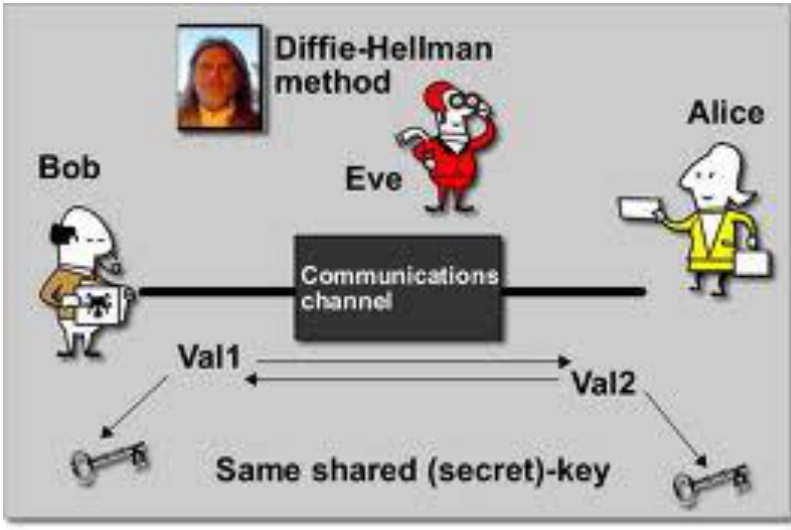
\includegraphics[width=86.52mm,height=145.83mm]{../../images/llm/page_008_img_01.png}%
\end{textblock*}

\end{document}
